\chapter{Design \& Implementation} % the next 4 chapters should be 40 ish pages

        
        

    \section{Introduction}
            The idea for this system was to create a website a user could interact with. To be able to make full use of the website the user should create a profile and rate a selection of movies. This will inform the recommender about their preferences. The user will participate in the debate and is shown a selection of movies from the local cinema. The recommender uses the information from the movies in the user's profile, as well as information about the recommended movies to create explanations that will be given during the course of the debate.

            Over the the project we created three systems. Each system was attempting to fulfil the same requirements although the first two were not successful, the third was. Each system was built on top of the previous using what was learned to create a better system. 

            Movies and their metadata are imported by the backend. Users sign up and create a profile this can then be filled with ratings. They can then start the debate. Movies are picked and their explanations created. The user can then participate in the debate by removing a movie after each round. Once this is completed they are left with one movie.


    \section{Schedule}
        At the start of the year, a set of goals for the project were laid out. The plan was to have the recommendation and explanations section of the project completed by the end of the first semester and to complete the debate and user interaction section in the second semester.\\


            \begin{tabular}{ |c|c| } 
                \hline
                September 27th      & Project started \\ 
                \hline
                October   10th      & Testing first system \\ 
                \hline
                November   20th     & Completed system to create explanations \\ 
                \hline
                November  30th      & Work slows in preparation for Christmas Exams \\ 
                \hline
                January 14th        & Start work on the debate and user interaction \\
                \hline
                March 1st           & Completed work on debate \\
                \hline
                March 10th          & Implement process for user trials\\
                \hline
                March 12th          & College Closed\\
                \hline
                March 26th          & Open Day (Cancelled)\\
                \hline
                April 1st           & User trials completed.\\
                \hline
                April 3rd           & Initial project end date (Postponed)\\
                \hline
                April 17th          & Project end as report due.\\
                \hline
            \end{tabular}
            
                    

    \section{First System}
        \subsection{Design}

            In this system, the user was presented with a command-line interface where the user would be asked which account to pick. These would be already existing accounts from the Movie Lens dataset. The system then picks 5 movies and gives back the average rating score for that movie. It would also search through the list of actors file and returns the actors that are linked to the movie. 
            It did give an explanation about a movie but was not based on a specific movie and was only one form of explanation and could not be easily extended. The interactions with the system from the user were limited to only supplying an already existing user id from the dataset. It was decided that actors was a good starting position for the movies and they are easily recognisable pieces of information about movies that people will cling to. For this project, we decided to use just user-supplied ratings from a dataset and the ratings users would provide during the use of the system. Other sources were considered, but implementing the collection of data from outside sources did not seem within the scope of the project, as the system only uses the fact the user has rated a movie, the ratings could be created from other data sources in an extended version of the project. 

        \subsection{Implementation}
            The first system was based of the Movie Lens and IMDB datasets. Movie Lens is a recommender website that suggests movies to users based on collaborative filtering of members' movie ratings. It was developed by GroupLens Research a research lab in the University of Minnesota. They offer a few different datasets. The first is a dataset designed for research that contains users with ratings on a scale of zero to five for a number of movies each. Each rating was a user id attached to a movie id and a rating. The dataset also contains a linking file between the movie ids that the Movie Lens dataset and the id system that the IMDB website uses. The movie ids from Movie Lens are not useful without the information to link them to the IMDB ids.
            
            The internet movie database referred to as IMDB \cite{IMDB} is the world's leading online repository for information about movies and other media. It launched in 1990 and is now owned by Amazon. It now contains over 6.5 million tiles made up of tv episodes, movies, video games and home media. It also contains over 10 million personalities. They supply subsets of their database online for people to use. We will be making use of the \textit{title.basic} and \textit{title.principals} datasets. These give information such as movie titles and their ids. It also gives actor information and links to the movies.

            This system would find some random movies from the dataset. Then for each movie it found it would get the average rating and also return the actors in it. For this we used the IMDB dataset. This contains a \textit{name.basics.tsv.gz} this contains 
            \begin{itemize}
                \item nconst (string alphanumeric unique identifier of the name/person) 
                \item primaryName (string name by which the person is most often credited)
                \item birthYear  (in YYYY format)
                \item deathYear (in YYYY format if applicable)
                \item primaryProfession (array of Strings)
                \item knownForTitles  movies the person is known for. 
            \end{itemize}
             A problem with this dataset is that it does not give all the movies the actor/actress was in only the ones they are known for, which reduces the usefulness of this. 

            \subsubsection{Development Tools}
                To start with the recommender only consisted of a command-line interface that was accessed by passing arguments to the Python scripts. This was sufficient for its purpose. Python was chosen for the project as we were familiar with it from previous assignments and a group project. It has many modules that can be imported to do anything that was going to be needed for this project. It is a general-purpose, high level interpreted language. The code produced is quite readable compared to other programming languages that we know. It is great for both small and large scale projects. It supports both functional programming and object-oriented programming, which we are going to use later in the project. It is dynamically typed and garbage collected. It also has a few other implementations that can be used for other advantages such as CPython which compiles Python code to bytecode for fast execution.
                
                We also started using Git which is a popular version control system developed by Linus Torvalds for use with managing the Linux Kernel. It designed for work in groups of people but is great for lone development as well. its goals are data integrity and speed and has support for distributed non-linear work. This is not a group project but I was working with multiple machines so having the git repo was very helpful. All code for the project was stored on Github which made working between machines possible. They provide hosting for software developers and were recently purchased by Microsoft. They also provide some code analysis which is useful for security vulnerabilities.
                
                Microsoft also makes VSCode which is a text editor come integrated development environment which has gained traction in the last few years. It was voted the most popular development environment in the Stack Overflow Development Survey where 50.7\% of respondents used the software \cite{StackOverflowDevSurvey}. It has built-in tools for git control and code completion. It also has a debugger that can be used with Python and Flask. 


            
        \subsection{Critique}
            This system was able to give explanations for the movies it was recommending to the user but the recommendations were not tailored and also not very relevant. The only information that the system would return is the average rating of the movie and the actors who appeared in it. This first system was a proof of concept and was used to learn about and get to know the two datasets. It was used to see what could be done with the datasets. This system did not meet most of the functional or non-functional requirements we had set out and so was used to form a new system that could be used to fulfil more requirements.
            This system was slow, had very limited user interaction as the user was just pretending to be an already existing user from the dataset and the presentation was lacking as it only have out information about actors.
                

        
    \section{Second System}
        \subsection{Design}
            After testing the usefulness of the data for explanations we decided we needed a way of creating them more easily. The initial idea for this system was to move to use a database to store all the information from the datasets this would speed up the access of the information in the system. The plan for the interactions was the same. The user would input a user id and would be given a set of actors based on information in their profile. A user would input a user id and the system would take this and compare this against ratings in the database. Taking all the movies from this user and then using the database to find all the actors for those movies. Ideally this would speed up the system and make it more useable. This system was going to be expanded to use all of the information that IMDB provide in their datasets; instead of just using actors to create explanations we were going to use more metadata about the movies. 

        \subsection{Implementation}
            Continuing on from the previous system, we wanted to implement something similar but with a database backend instead of searching the files. Keeping the same front end of inputting a user id and searching for some actors. Initially we started implementing SQLAlchemy models for each object in the system. The movies table was made up of 
            
            \begin{itemize}
                \item id       - INTEGER
                \item movie id - INTEGER
                \item name     - VARCHAR
                \item rating   - FLOAT
                \item IMDBid   - VARCHAR
            \end{itemize} 
            below you can see this translated into SQLAlchemy \ref{MovieClass}. This is a Movie class that can be instantiated in the code to create a new movie and then saved to the database as an item in the movies table. 
            

            \begin{lstlisting}[gobble=16, tabsize=4,caption=Representing the movie class,label=MovieClass]

                class Movie(Base):
                    __tablename__ = 'movies'
                    id = Column(Integer, primary_key=True)
                    movie_id = Column(Integer)
                    name = Column(String)
                    rating = Column(Float)
                    IMDBid = Column(String)

                    def __repr__(self):
                        return "movie_id='%i' name='%s'" % (
                            self.movie_id, self.name)
            \end{lstlisting}

            A similar thing was also implemented for some of the objects we were looking at putting in the system. An actor class was created with similar attributes swapping out IMDBid with the actor id and removing rating. This was then linked to the movie class using the class depicted in ~\ref{ActorToMovieClass}

            \begin{minipage}{\linewidth}
                \begin{lstlisting}[gobble=20, tabsize=4,caption=Representing the Actor to Movie class,label=ActorToMovieClass]

                    class Actor_to_Movie(Base):
                        __tablename__ = 'actor_to_movies'
                        id = Column(Integer, primary_key=True)
                        actor_id = Column(String,ForeignKey('actors.actor_id'))  # nconst 0
                        movie_id = Column(String, ForeignKey('movies.movie_id'))  # tconst 0

                        def __repr__(self):
                            return "<Movie_to_actor_paid(id='%i', actor_id='%s', movie_id='%s')>" % (
                                self.id, self.actor_id,self.movie_id)
                \end{lstlisting}
            \end{minipage}


            SQLAlchemy is an object-relational mapper which allows you to create an interface between items in a database and the objects in Python. Having developed with SQLAlchemy for our group project before it made sense to use it again for this project. This gives an interface in Python that can be used to create, edit, delete and search for items in the database using objects in Python. The problem with our use of this was that creating thousands of objects for inserting was going to take a long time. The plan was to take each piece of metadata and create a new Python object that would use SQLAlchemy to map to a table in the database. These classes have methods that can be used to add , update and remove each one. 
            


        \subsection{Critique}
            This system was not fully implemented as inserting the data from the datasets using SQLAlchemy was going to take a prohibitive amount of time. Instead, we moved onto system three which was also the final system. While using the IMDB dataset parsing all the files and linking the data became difficult so instead we moved to a different source of the information. 

        
    \section{Third System}
            \subsection{Design}

                The third system is made up of three parts. The first is obtaining movies and the data and importing it into the database. Next is taking that information and creating explanations with the movie and user information. In the third section, we will describe the user's interactions with the system and how it was presented to the user.


                \subsubsection{Collecting Movies}
                    In this system, we were continuing to use the user ratings from the movie lens dataset. These needed to be imported into our new database. We were unable to use the IMDB datasets as they do not contain all the information that we would like. Instead of using the IMDB datasets directly we are using the \textit{Open Movie Database}. This is an API created using some of the IMDB data as well as other sources. We were able to request data from this API to use. Combining the user ratings and the information from the API we were able to create a database of movies that we could create recommendations from. The application programming interface given by the Open Movie Database lets users specify the information required in the responses. 

                    The movies we are recommending in this system can come from two sources. Either they can come from the local cineplex or they are movies we are recommending to them based on their neighbour's ratings. Depending on the current debate we can either find the names of the movies from the local cinema by scraping the data or we can calculate which movies to recommend based on the user's Pearson coefficient between them and the other users in the system. As explained in \ref{sec:pearsonCorrelation} the Pearson correlation can be used to measure the similarity between two users. This is a form of collaborative filtering and can be used to get movie recommendations for users. We decided a choice many people have to make is what movie they want to see at their local cinema.The data that is collected from this section of the design can then be used to create explanations and debates.


                \subsubsection{Creating explanations}
                    After collecting movie information from the data sources and storing it. We need a system to create explanations. Based on the ratings that a user has we take every movie in their profile and collect all the common pieces of metadata between these movies and the movies that we are recommending. We gathered them we get the count of the number of times each piece of metadata appears in the user profile, this contributes to scoring the item. This creates a list of explanations we can give to the user. These are then scored and stored in the database. The scoring is done differently for each piece of metadata. 


                    Another form of explanation that the system uses is your neighbour's ratings. We calculate a user's top 50 neighbours based on the comparison between the user's ratings and the ratings of every other user in the system. Once a list of neighbours is created we can take the top 50 and show the ratings those users gave the movie we are recommending. Depending on the piece of metadata the scoring is done by comparing how often an item appears in the database of movies in the system versus how many times it appears in the user's profile. The higher the better as we are assuming for example that if a user has seen an actor in many films they might be likely to want to see them again. 


                    \subsubsection{User interaction}\label{sec:3UserInteractionDesign}
                    To interact with the system the user will go to one of a few pages after they have created an account and logged in. There is a page where a user can import a new movie by supplying its name or IMDB id and give it a rating on that page. This will use the importer to import the movie and add the rating to the user's profile. There is also a page to rate any existing movie in the system. The user is presented with a selection box of all the movies in the system and another to select a rating between zero and five. If the user has already rated the movie we update their rating. On this page are the controls for the user trials and the debates. The user can start the user trials. This has six rounds, each has different settings for creating recommendations and explanations. The user is able to start the trials and advance them from this page. There is also the showings page which was used for testing. This page lets the user see all the current movies and all their explanations attached without needing to go to the debate.

                    Initially, the user trials were going to be done in person, where we could change the settings as the user completed debates. As the College was closed due to the COVID-19 pandemic, a new system had to be created. The user trials are explained in chapter \ref{sec:userTrials} The final page the user can visit is the debate page. On this page the user sees the six movies that are being recommended to them along with the explanations underneath. The movies are represented by their title and a poster.  There is a movie selection box at the bottom of the page that lets users remove a movie each round. The system will also need to be hosted so that users will be able to access it. The plan is to host the system publicly from home as this is the cheapest and easiest method. 

        
                    \begin{figure}
                        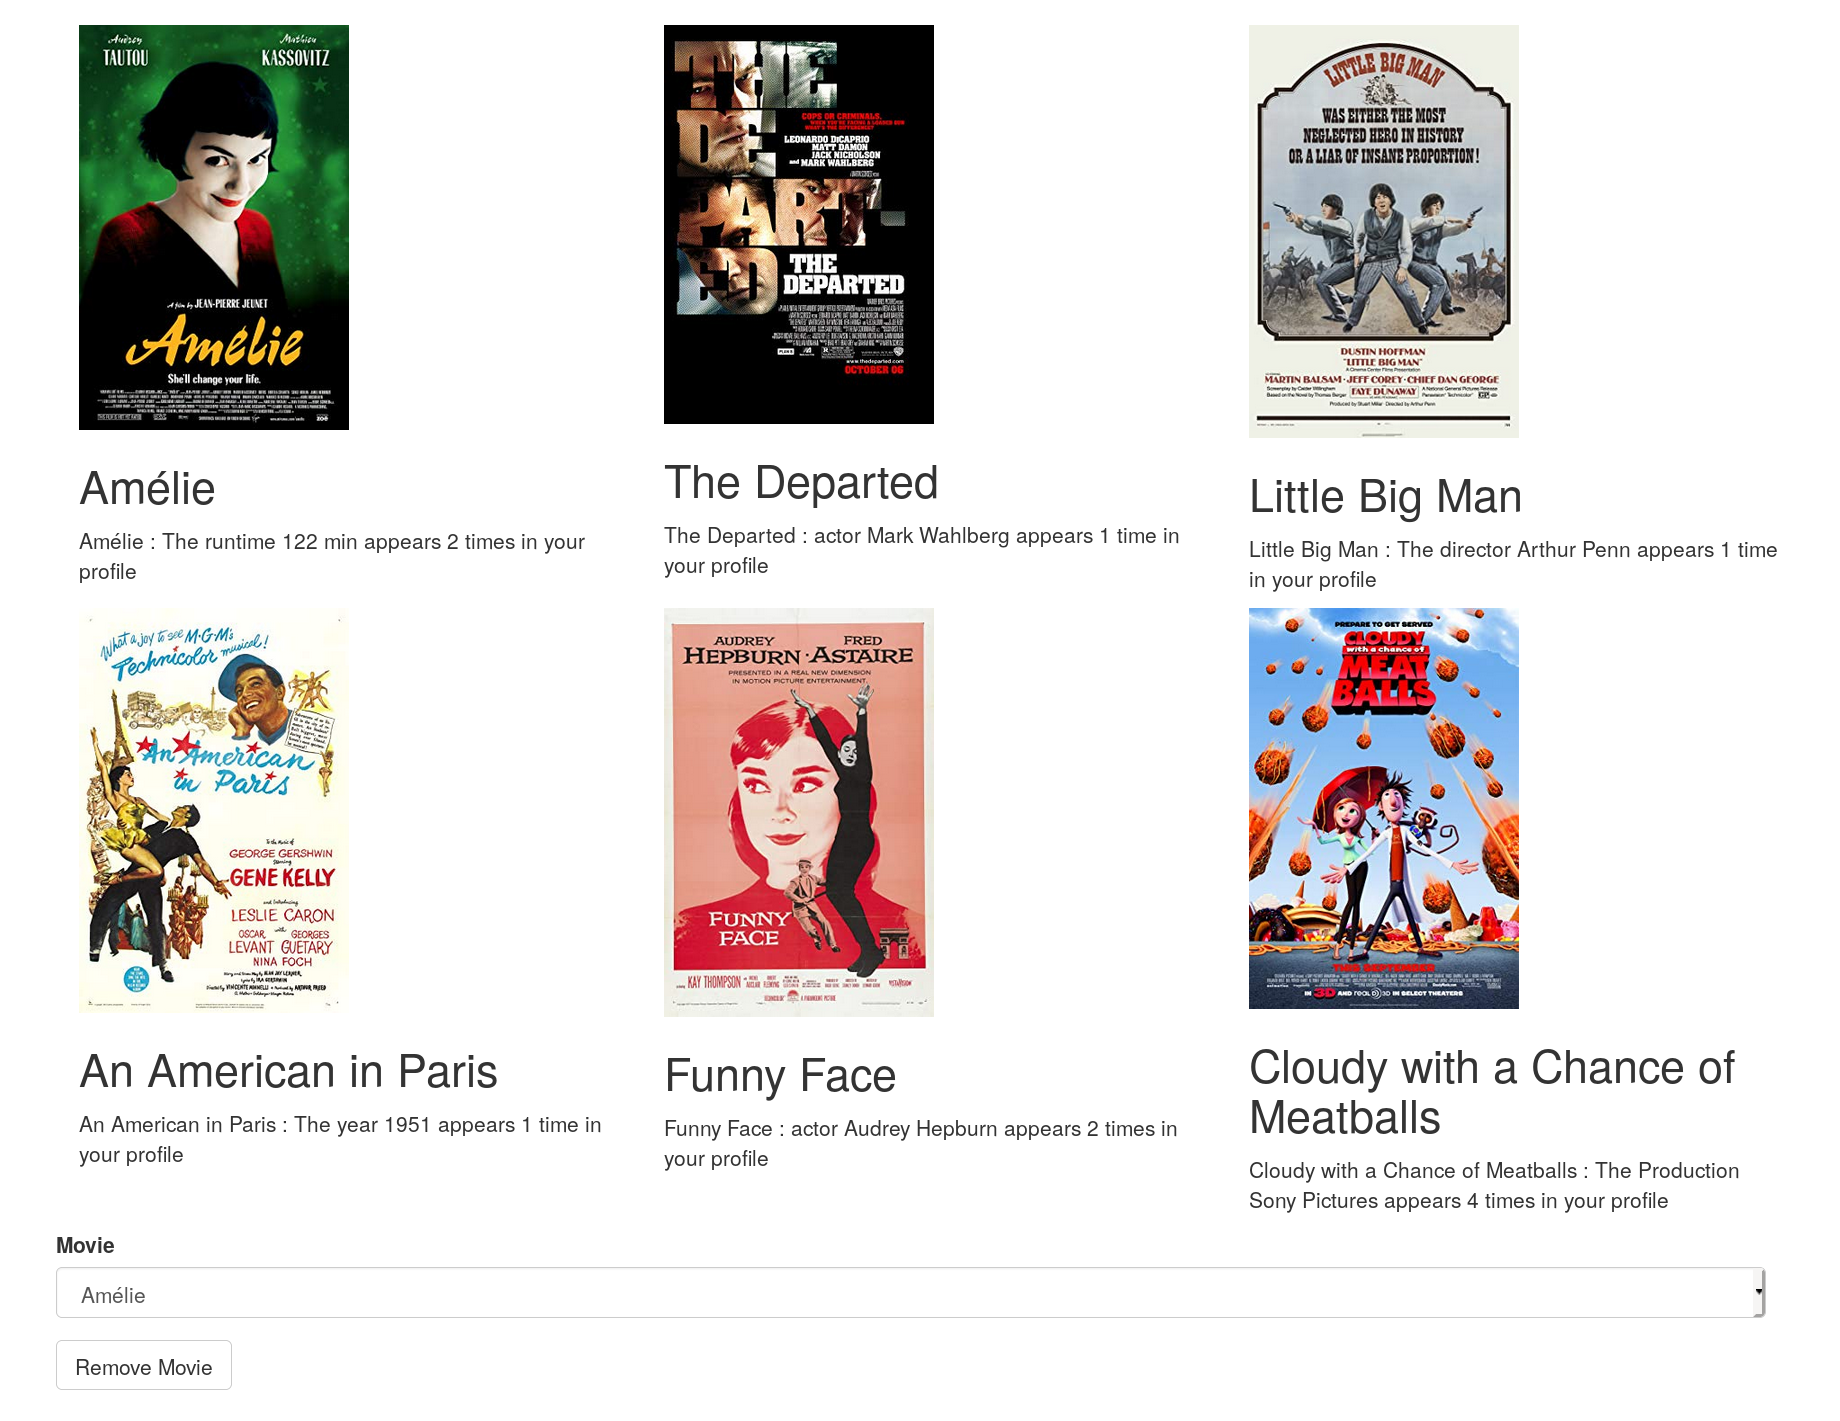
\includegraphics[width=125mm,scale=0.5]{system1.png}
                        \caption{The debate screen of the application}
                    \end{figure}

        
                    \subsubsection{Critique}
                        Ideally the system would not use just a user's movie ratings. It would use some less specific ratings of a system. \cite{10.1145/1555400.1555432}. In this paper, it is seen that users are likely to not want to rate movies explicitly. If the system was used inside another system, the user preferences could be calculated based on things other than ratings. Such as the watch list of a user or the movies they have looked at on an interface but not watched. We could also deem a negative rating of a movie a user started to watch but stopped and never came back. To create explanations we just looked at all of the movies a user had rated and took objects they had seen frequently and explained the recommendation using these. The scoring of these explanations did not take into account if the object was taken from a movie the user disliked. The scoring for explanations could have been made better if it took into account the actor they that was being used as an explanation was from a movie the user did not like.

            \subsection{Implementation}
                \subsubsection{Collecting Movies}\label{sec:CollectingMovies}
                    To be able to create recommendations and explanations we were going to need a database of movie information. Instead of using the IMDB datasets which do not give the information we want. The information we would like would have to be created by a system we create.  We started using the Open Movie Database API. 

                    "The OMDb API is a RESTful web service to obtain movie information, all content and images on the site are contributed and maintained by our users."\cite{OpenMovieDatabase} This can be accessed online or through one of a few different Python wrappers. You can supply an IMDB id or a title and it will give you back structured data about the movie similar to what the IMDB datasets can provide but easier to parse. This gives more information than IMDB provide in their datasets and also gives posters. The user can then specify what type of content they want from the API with different parameters when they make the request. There is a module that has been created called OMDb \cite{pythonOmdbApi}

                    As part of wanting to create the database for user and movie information we needed to decide on which database to use. There are many options for this. We decided on using SQLite. It is a relational database management system that instead of using the standard client-server model, it instead uses a function library that can be called from the application. SQLite is file-based. SQLite is considered simpler than MySQL which is a standard client-server DBMS. Using MySQL would have increased the complexity of the project. It would have involved running a MySQL server alongside the application. MySQL can be much faster in some cases but through the use of SQLite transactions we can reduce the difference and make SQLite faster. Another popular option is PostgreSQL which is open source and has some advantages like the ability to deal with a great number of concurrent clients. 

                    In order to collect movies, we can take a movie id from the movie lens user ratings and query the api and it will give us back JSON that can be split up and inserted into the database. Each object has its own table, for example actors and directors. These are all represented as an object id and a string. There is a table that shows, for each movie, all of the objects attached to that movie. The code in figure \ref{lst:InsertingMovies} shows how we take the information that the OMDb Python library returns and use it to create new objects. 

                        \begin{minipage}{\linewidth}
                            \begin{lstlisting}[gobble=32,tabsize=4,caption={Importing movies into the database},label={lst:InsertingMovies},language=Python]
                            
                                def import_movie(IMDB_id):
                                    json_for_movie = omdb.IMDBid(IMDB_id)
                                    response = literal_eval(json_for_movie)
                                    movie = response["IMDB_id"]
                                    for object in response:
                                        if check_exists(object):
                                            pass 
                                        else:
                                            create_object_and_insert(object)
                                            create_movie_object_link(object,movie)
                            \end{lstlisting}
                        \end{minipage}
                      

                    The names of movies that are going to be recommended can come from two sources. The first is movies that are being shown at the local cinema and the other is movies the user's neighbours have rated highly. 

                    In order to get a list of movies from the local cinema we create a function \textit{get\_omniplex\_movies()} . This would make requests to the website and retrieve a list of movies formatted in such as way that would be usable to us. We used the Python requests module to make requests to the website. The website would not return a list of movies unless we used a valid request with the correct headers. We included the standard headers that would be given if you were using a web browser to access the page and retrieved the list of titles that were needed. This cinema has showings for more than just movies so these needed to be filtered out manually as there was no way to request just a list of movies that would work with the system. This was done mainly as the API we were using for movie metadata would not contain these other showings. We would therefore not be able to make explanations for them so they were excluded. \textit{Beautiful Soup 4} was used to parse the returned HTML. This is a Python library for pulling data out of HTML and XML files. It provides an easy way to parse the HTML. 

                    
                    To calculate a users neighbours we used the Pearson correlation coefficient. Using this we can get a measure of the similarity between two user's ratings. Initially, we were going to create neighbours based on the threshold of the relationship between them but a better practice is to use a limit on the number of neighbours and for example take the top 30 nearest neighbours. \label{sec:CreateNeighbours}

                    \subsubsection{Calculate Pearson Coefficient}
                
                        To calculate the Pearson coefficient for our users we used the Scipy stats module. This provides a function \textit{pearsonr(a,b)} which takes in two lists and returns the coefficient and the p-value. If either of the lists is a list composed of all the same values the function will return nan. This is because you cannot calculate variance in a list of the same numbers as they do not vary which would lead to trying to divide by zero in the formula. In our implementation, we assumed the coefficient was zero between two lists if one of the lists was composed of only one value repeated.
                        
                        First the function in \ref{fig:FindingNeighboursPearsonMethod} finds all of the possible neighbours. This is anyone who has rated at least one movie that the user has also rated. Then we find every movie a possible neighbour and the user share. When run, the SQL shown in \ref{fig:FindingNeighboursPearsonMethodSQL} returns a list of pairs of ratings. Each pair is the rating for a movie that is shared between two users. The pearson correlation is calculated between the two lists. This is done for each neighbour and the results are sorted and ranked. The fifty neighbours with the highest correlation with the user are used as the neighbours.

                        Assuming $\bar{x}$ is the mean of list x , $\bar{y}$ is the mean of the list y and that $s_x$ and $s_y$ are the std deviation of list x and list y you can use these to calculate the coefficient. For each value in each list, you need to calculate a standardised value using $(z_x)_i$ and $(z_y)_i$ for lists x and y respectively. For  each of the standardised values you can multiply them together then add them together and divide by n-1 where n is the length of the lists. This results in the Pearson coefficient between lists x and y.

                        \begin{minipage}{\linewidth}
                            \begin{lstlisting}[gobble=30, tabsize=4, caption=SQL used to find neighbours ratings. ,label=fig:FindingNeighboursPearsonMethodSQL]

                                common_ratings_for_neighbours = "SELECT a.rating , b.rating  from (" \
                                "SELECT rating, IMDB_id from user_ratings \
                                WHERE user_id == ?)a JOIN (SELECT rating, IMDB_id from " \
                                "user_ratings where user_id == ? )b ON \
                                a.IMDB_id == b.IMDB_id"
                            \end{lstlisting}
                        \end{minipage}
                        


                \subsubsection{Creating Explanations}                

                    In the third system, we wanted to create a plan for how to add more explanations over time. In the first two systems they were only able to accommodate actors and adding any new explanation types would be difficult. We needed a system that would be extensible to our needs. It was decided to make a database table for each explanation type and link them with a joining table. This was unable to be done with SQLAlchemy and this was part of the reason for the move to using plain SQL. Each explanation type would get what is shown in \ref{fig:dbLink2}. This would let us compare objects between movies easily. If we wanted to add another explanation type it would just mean using the existing code with another table. 
                    
                
                    \begin{figure}[H]
                        \begin{center}
                        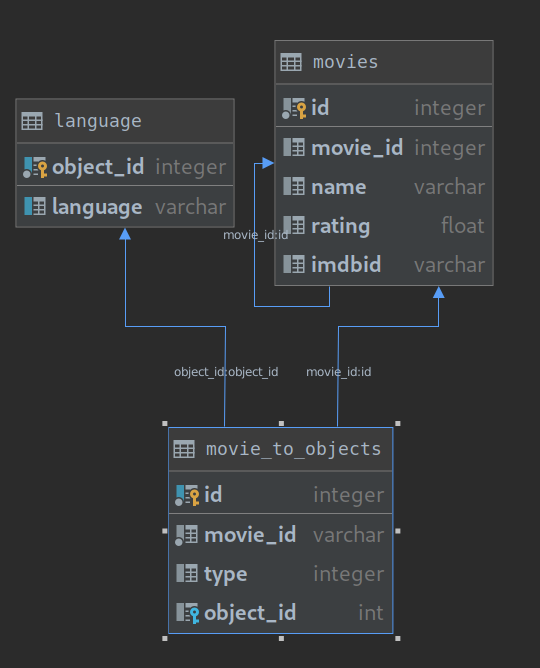
\includegraphics[scale=0.25]{dbLink2.png}
                        \end{center}
                        \caption{Database Implementation}
                        \label{fig:dbLink2}
                    \end{figure}
                    

                We also had to move to use the SQLite3 module as although using SQLAlchemy meant we had easy to use Python objects. Creating a Python object for every line in a table is a slow way of adding things to a database and would be too slow to continue with. The API that was explained in \ref{sec:CollectingMovies} returns a number of pieces of metadata. We turned some of these into explanations. Below is a list of items that can be used as explanations:
                \begin{itemize}
                    \item Actor
                    \item year 
                    \item director
                    \item genre 
                    \item rated (The MPAA rating system)
                    \item released (Year of release)
                    \item runtime 
                    \item writer 
                    \item language 
                    \item awards (Any awards the movie has won)
                    \item productions (The production studio that made the movie)
                    \item country
                \end{itemize}
        
                The code shown below in figure \ref{fig:CreatingExplanations} shows how the system takes objects from the \textit{movie\_to\_objects} table and creates results that we can use in creating explanations for each user. This needs to be done for each movie that is being recommended. This returns the result from the SQL query which is then used to make an explanation object for each item returned. When creating them they are scored based on the number of times they appear in your profile or random depending on whats needed. When creating the debate the explanations with the highest score are picked. They are given a score between 0 and 1. In figure \ref{fig:ScoringExplanations} we show how some of the explanations are scored. As part of creating the explanation objects they have a number of methods that are used in their creation. It was decided that using the SQLite3 module instead of using the SQLAlchemy would work better because the below statement would have been much harder to create using SQLAlchemy. Each object in the database which is a piece of movie metadata is represented by an object id and a type. Each type has its list of objects. For example actor Tom Hanks has object id 792 and is of type one. We have an enum representing the different objects that exist so they can easily be referenced.
                
                
                    \begin{minipage}{\linewidth}
                    \begin{lstlisting}[gobble=20, tabsize=4, caption=Code used to retrieve data for explanations,label=fig:CreatingExplanations]
                    def compare_movie(IMDB_id, user_id):
                        c,conn = get_db()
                        query = """
                        SELECT  t1.type, t1.object_id , COUNT(*)FROM (
                        (SELECT movie_id,type,object_id FROM movie_to_objects
                        WHERE movie_id == ?) t1
                        LEFT JOIN
                        (SELECT movie_id, type, object_id FROM movie_to_objects  GROUP BY
                        object_id, type , movie_id HAVING movie_id in (SELECT IMDB_id FROM
                        movie_id_to_IMDB_id
                        WHERE IMDB_id in (SELECT user_ratings.IMDB_id FROM user_ratings WHERE
                        user_id == ?))
                        ) t2 on t1.object_id = t2.object_id AND t1.type = t2.type) GROUP BY
                        t1.type, t1.object_id ORDER BY t1.type;
                        """

                        c.execute(query, (str(IMDB_id), int(user_id)))
                        result = c.fetchall()
                    \end{lstlisting}
                \end{minipage}

                    \begin{minipage}{\linewidth}
                        \begin{lstlisting}[gobble=24, tabsize=4,  caption=Code used to rate an explanation, label=fig:ScoringExplanations]
                            def get_score_for_type(self):
                                max_for_type = get_max_for_type(self.explanation_type)
                                min_for_type = get_min_for_type(self.explanation_type)
                                normal = (self.count - min_for_type) / (max_for_type - min_for_type)
                                return normal
                        \end{lstlisting}
                    \end{minipage}

                As an alternative to the above explanations we did create some more examples of explanations but they did not get used in the system that we built. An example of this is shown in figure \ref{fig:past_performance}. This method takes a movie as input and will return the average rating of the movies the director has directed. It ended up not working with the system that we implemented but it could have been worked on in the future.


                    \begin{lstlisting}[gobble=20, tabsize=4,  caption=Code used to get the past performance of the movies of a director,label=fig:past_performance]
                        def past_performance(movie_id):
                            query_for_director = """
                            SELECT SUM(rating)/COUNT(rating) FROM movies_2 WHERE IMDB_id in (
                            SELECT movie_id from movie_to_objects WHERE \
                            object_id == (SELECT object_id from
                            movie_to_objects WHERE movie_id == ? AND type == \
                            3) AND type == 3);"""
                            
                            c.execute(query_for_director, (movie_id,))
                            response = c.fetchone()
                            if response is not None:
                                return response[0]
                            else:
                                return None
                    \end{lstlisting}

            \subsubsection{User Interaction}

                The first two systems were only usable on the command line where you would supply parameters and it would give you back information. As we wanted to create a whole debate system with user trials we needed something more interactive. We decided on a website using Flask. Flask is a micro web framework that can be used with Python. We had previous experience with it from a group project so it seemed like a good choice. There are other similar options out there like Bottle. Flask does not require you to use certain tools with it. You can use whatever you like. We will talk about reasons we picked Flask more in a later section \ref{sec:webDevelopment}
                
                As part of the requirements, we needed the user to be able to input information such as movie ratings. We created four main pages. 
                The showings page was used for testing before we created the debate. This page shows the current movies for a user and all of the explanations for those movies. The ranking page contained the controls for the debate and user trials and gave the user the ability to add ratings to movies in the system. When the user gave a rating we would get the data that was returned from the Flask form and we used the function \textit{rate\_movie(user\_id, IMDB\_id, rating)} to update the \textit{user\_ratings} table with the new information. This either involved finding the existing rating for that movie or creating a new row with the IMDB id and the rating. We also have a page that would let a user take an IMDB id of a movie they wanted to rate and it would import the information about the movie into the system like explained in section \ref{sec:CollectingMovies} 
                
                The controls of the debate and user trials could be used to create a new debate, start a new user trial or reset an already existing one. The last page we had was the debate page. This would be used after a user had created a debate. It would show a set of movies and their explanations and would update at the end of each round of the debate. The debate page like other pages had the nav bar at the top, along with the six posters for movies we would be recommending and their explanations. Below that we had a selection box that allowed the user to remove a movie.

                Initially the plan was for a user to rate movies and then create a debate which could be stored in a JSON format to be used later. When the user created the debate, it would pick a set of movies as explained above and it would create explanations. The system would then store the JSON using the function \textit{write\_to\_json}. This would accept a JSON dictionary and write it to a file to be accessed later. When the user accessed the page for the debate we would then retrieve the debate using this file and show it to the user. At the end of each round, the JSON would be updated by removing the chose movie along with its explanations. 

                Instead of continuing to store the program's state in JSON we moved to using the database. This was necessary as we started to work on Implementing the user trials. We would need to keep track of what round each user was on and their debate. When the user creates a debate we store the movies that were selected in the database along with the explanations for those movies. This involved creating a new table to store created explanations for each movie and a table for the movies the user was to be recommended. The explanations were stored in the form:

                \begin{itemize}
                    \item id (the distinct explanation id for the database)
                    \item user id (the id of the user who created the debate)
                    \item IMDB id (the movie id the explanation related to)
                    \item count (the number of times the object appeared in the user's profile)
                    \item type  (the type of object this was e.g. actor or director)
                    \item object id (id of the object in its respective database table)
                    \item explanation string (the explanation given to the user in the debate)
                    \item rating (the rating the explanation was worth)
                \end{itemize}
                
                The soon to be recommended movies for a user were stored with:
                \begin{itemize}
                    \item id (the distinct id of the relationship between this movie and the user)
                    \item user id 
                    \item IMDB id 
                    \item movie title
                    \item poster filename (where the poster is stored in the system)
                    
                \end{itemize}

                These two tables can be pulled from to form the debate. When the users goes to the debate page the system finds the current movies they are to be shown for that user. The round of the debate and the user trial was also stored in the database for each user. Based on the round of the debate the system picks explanations for each movie. The debates start with one explanation per movie and each round adds one for each movie. At the end of each round the user removes a movie this movie is then removed from the \textit{current\_movies} table for the user so it will not be included in the next round. 
                
                The user trial has six rounds which are split in half. Each debate in the user trials has different modifications applied to it. The round of the user trial is checked when creating the debate. This is then used to determine three settings. The first is which movies to recommend either, movies from the cinema or movies from the Pearson calculations. This setting is inactive for the first three rounds but is activated for the last three. The setting being inactive means we take movies from the local cinema and active means we take movies from the Pearson calculations. The second is whether the user sees a poster and movie title with the explanation. The final setting is whether the explanations are created with our custom scoring function specific to the explanation type or assign a random score to each explanation. We had a function \textit{return\_settings} that would return a triple of settings based on the user trial round. As part of moving the debate and user trials we created a suite of methods that would manage the inserting updating and removing of debates and user trials from the database.
                
                
        
                \subsubsection{Presentation}\label{sec:webDevelopment}


                    As we mentioned above we are using Flask to create the website. Flask routes allow you to map urls onto Python functions. When a url is visited the function matching that is run. For example our system has a route for any GET or POST requests that come to \textit{/user/<username>/debate/} will run the \textit{debate\_page()} function. In this function, we can call other functions to create a page and then at the end we can use \textit{render\_template()} to return content that will be used in the Jinja template.

                    Jinja is a web template engine designed to be used with Python. it uses text-based Python like expressions. Its the default template engine for Flask and it integrates well with it. it allows us to define templates for pages programmatically without writing HTML. It also integrates well with Flask forms which only requires on line to create and show the forms on the page. It also allows the use of base templates that can be included in other which reduces the reuse of code between pages. Base templates are extended to create the new template. These are useful for containing style sheet links and navigation bar html\ref{fig:JinjaTemplate}
                

                    \begin{lstlisting}[gobble=20, tabsize=4,  caption=Jinja template example, label=fig:JinjaTemplate]
    
                        
                        
                    
                        
                        <h1>{{ _('Rank movies') }}</h1>
                        <div class="col-md-4">
                            {{ wtf.quick_form(form) }}
                        </div>
                        
                        \end{lstlisting}

                    One of the reasons we tested out using SQLAlchemy was because there is a version called Flask-SQLAlchemy that can be used with Flask. It also supports the use of WTForms which is a library for quickly creating web forms. Flask lets us easily create pages for the project. We can define the location of the page using the code shown in \ref{fig:CodeToCreatePage}


                    \begin{lstlisting}[gobble=20, tabsize=4,  caption=Code to create page, label=fig:CodeToCreatePage]
                        @app.route('/user/<username>/rank/', methods=['GET', 'POST'])
                        @login_required
                            def rank(username):
                                form = debateForm()
                                return render_template('recommender/rank.html', user=username, form=form)
                    \end{lstlisting}

                    In the page function we can retrieve what is going to be shown on the page for the user and then pass that as parameters of the function. In this page we are using a Flask form that accepts the user rating for a movie. In the debate page a JSON object is created that contains the movie title, poster and the explanations. This is returned in the render template function. The jinja template created for the debate page then parses the JSON and shows the movie and explanations. To update the debate each round we can just change what gets passed into the jinja template. 

                    
                    One of Flask's best features is the ability to create a development web server that can be used for rapid prototyping. When using the production Flask web server, it has to be restarted every time a change is made in the code for it to be represented in the system. This makes sense for production where you would not like your web sever to restart suddenly when a developer makes a change. On the other hand the development server will automatically restart when it detects a change in the code which speeds up development as it takes much less time to make a change and see it represented. This also integrates with Visual Studio Code's development workflow and the debugger in can be setup to walk through the code and add breakpoints to inspect variables as the code is run. This is incredibly useful during development. When finished developing and moving the website to production it is advised to move away from using the built-in web server and instead use a production-ready one.

                    Another advantage of Flask is its ease of use. When developing we used \textit{Flask-Bootstrap} for the look and feel of the website. This is an extensions that consists mostly of a Flask blueprint that makes it easy to use the Bootstrap front end library with the project. It automatically applies a default CSS to the website when included. This was enough for us as the appearance of the application was not what we were going to spending time on. When we started to do user testing we realised that because we used Flask and Bootstrap the website worked perfectly when used on mobile devices. Flask Blueprints allow a developer to separate their code into modules. This is great for a large project. We had a separate blueprint for our login system. We were able to separate that code out into its own folder where we could create a set of routes that are accessed from the main application. They can be accessed from the main application once they are registered. 
                    
                    Gunicorn is a Python Web Server Gateway Interface HTTP Server. It is built to have many different web service interact with it as long as they use this gateway interface. The WSGI is a way to make sure that web servers and Python web applications can easily talk to each other. The web application can be created by Gunicorn and used to handle more requests. There is an alternative to Gunicorn called uWSGI that does a similar job. We did not have many static pages in our application so we did not use a web server. Nginx is an example of one of these. We would not be serving many people or static pages so it was not required that we use one. This would be inefficient for a larger scale application as Nginx is developed to serve more users and static pages at the same time which is helpful. This web server would stand between the Flask application and Nginx.

                    Docker is a containerization platform that allows developers to isolate their application from its environment. It lets the developer package the application and all of its dependencies into one container. This allows us to redeploy the application easily to different places that support Docker containers. Which is any Linux Server with the docker software installed. They use OS-level virtualization to host applications. This means all docker containers on a host run on the one operating system reducing the amount of computation needed compare to a standard virtual machine. 
                    
                    Initially we used a single Dockerfile to contain all the configuration for our application but we moved to using Docker Compose instead as it allows us to integrate with Traefik which would reroute our web traffic to the application running on the server. This routes traffic received on ports 80 or 443 to a specific docker container based on the url specified. This is useful if you are running multiple services on one machine which docker supports. 

                    A domain was purchased to be used with the application. Using Cloudflare DNS this let us point the domain at the static IP address of the server. Any Traefik bound for our application would then be checked by Cloudflare for malicious intent before it reached the web server. After it had routed through Cloudflare and it reached the server it would be sent to Traefik which would take any traffic for http://recommender.domain.xyz it will route that traffic to the docker container running the Gunicorn server hosting our application. 


                    \subsubsection{Critique}
                        Implementing the storage of the explanations in a JSON file seemed fine at the time but expanding it out for use with the debate was over complicating the program. It would have been better to move to using a database to store the state of all of the application's states earlier in the project.
                        As we will mention in the evaluation chapter \ref{sec:userTrials}, there were some bugs in the system that could have been fixed with a better testing plan. Even though the database is more extensible that the methods we used in previous systems there are still ways to improve it such as making it more generic to the type of data being used. 



            \subsubsection{Data Flow Diagram}
            \begin{figure}
                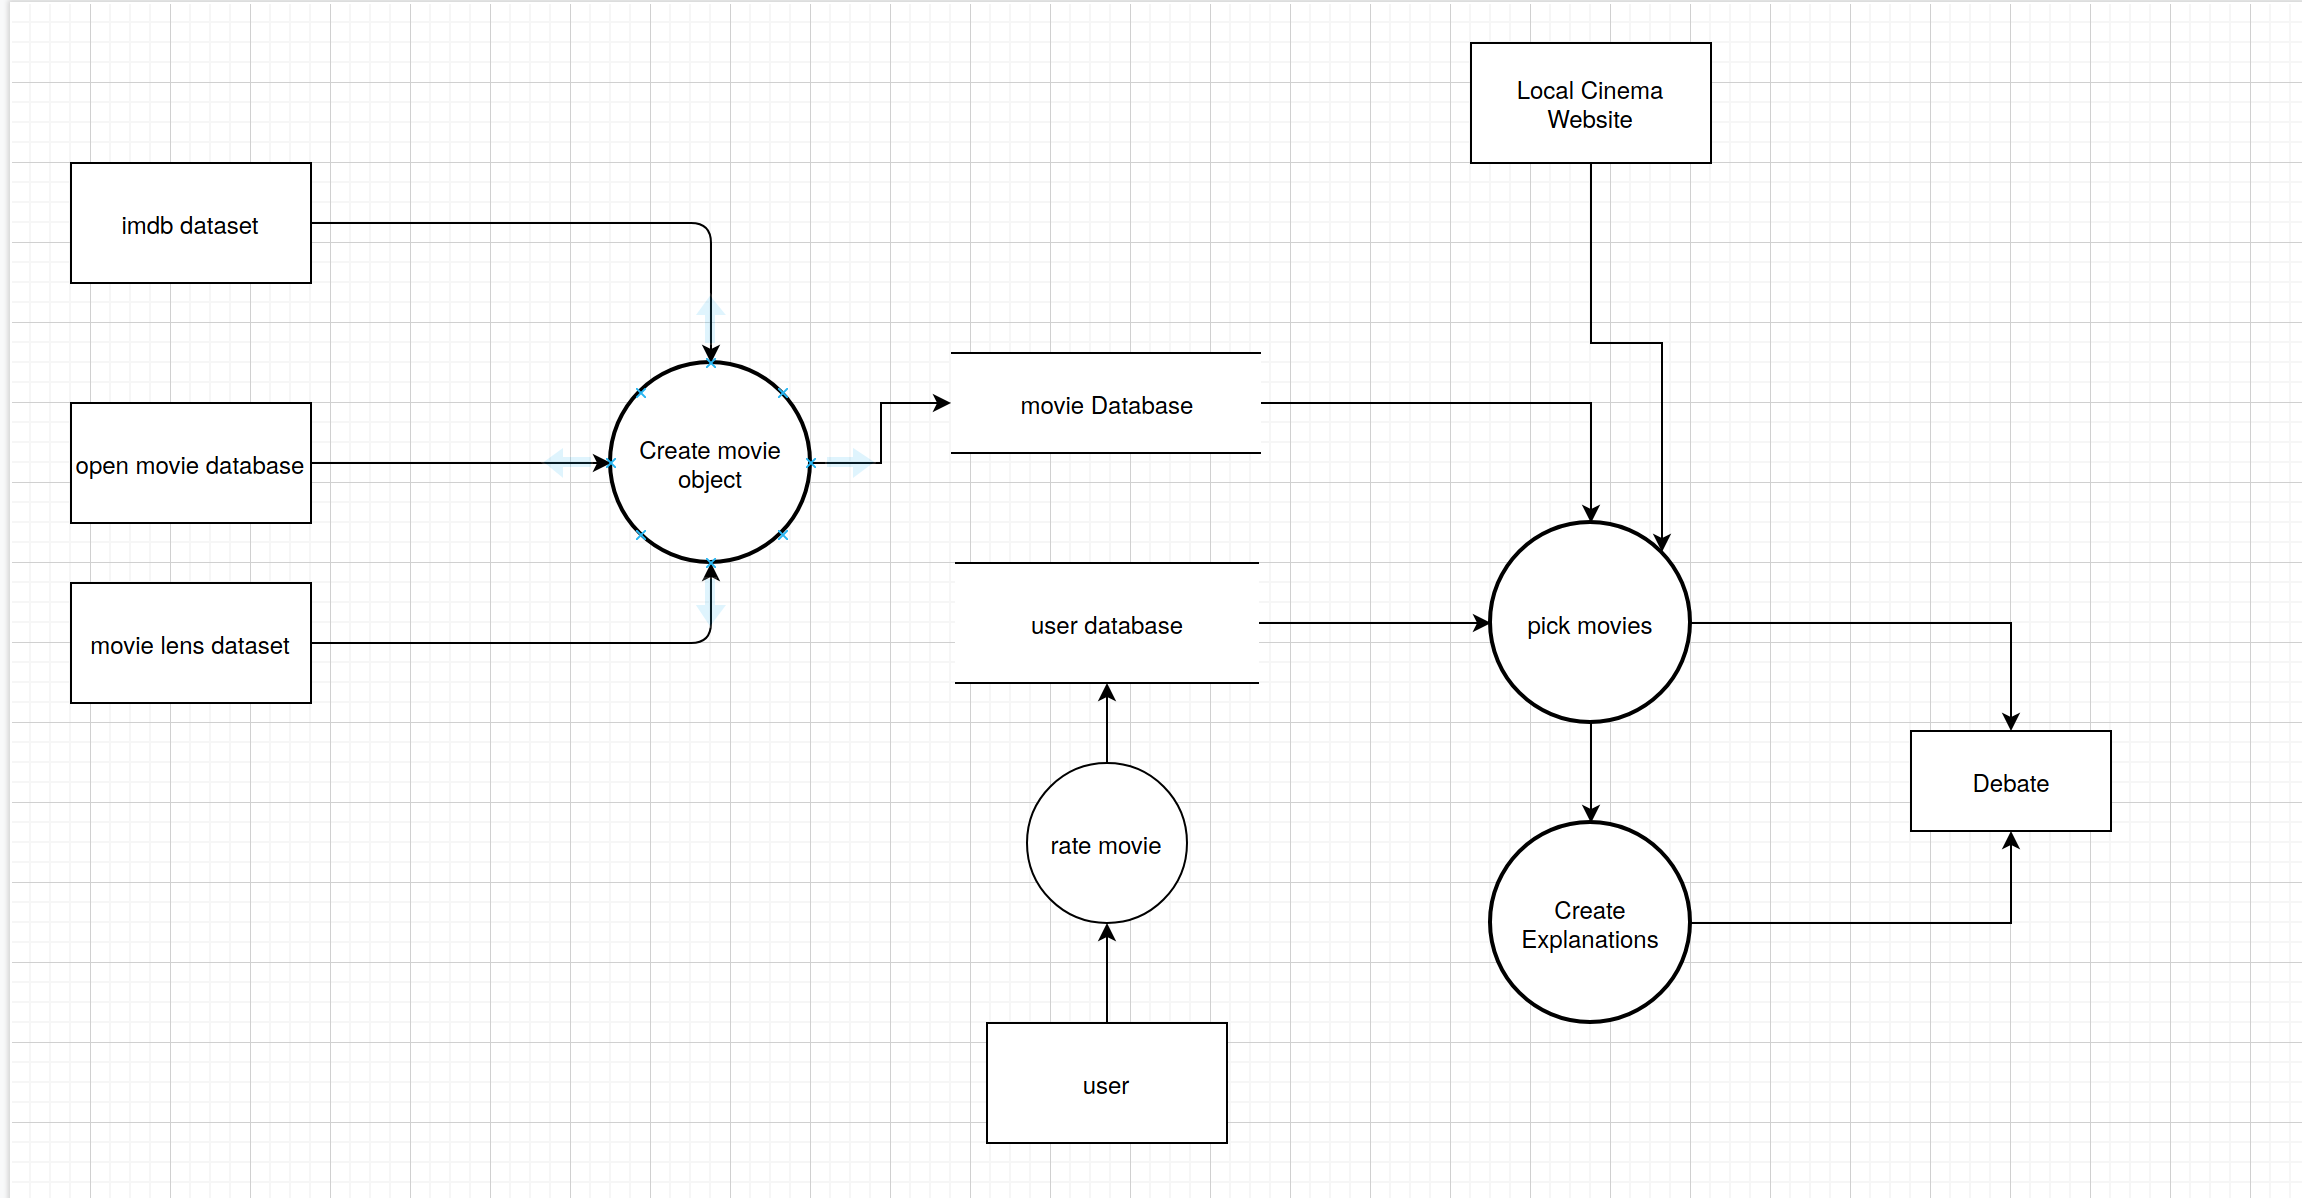
\includegraphics[width=100mm]{DataFlowDiagram.png}
                \caption{Data Flow Diagram}
                \label{fig:DataFlowDiagram}
            \end{figure}
            
            As shown in figure \ref{fig:DataFlowDiagram} the data comes in from the open movies database and gets turned into database objects. User ratings from the movie lens dataset gets put into the users\_ratings table. when creating the debate the movie titles that are going to be recommended get taken from either the user database in the case of movies recommended by neighbour or from the local cinema. These are then used with the movie objects database to compare movies. Explanations are created this data and shown to users in the debate. 


            \subsection{Example}
                In our final system we are able to give the id of a movie into our system and it will get all the objects that are related to that movie and cache them. For example let us look at the movie Iron Man (2008) which is represented by the IMDB id \textit{tt0371746}. It will first get passed to the function \textit{scrape\_omdb\_with\_movie\_id(imdb\_id)}  which will take in an IMDB id which are of the form tt then seven or eight numbers. This function will consume the JSON response from the OMDB API shown in Appendix \ref{fig:ironmanjson}. This is then passed to the function \textit{filter\_movie(response)} which looks at each section of the JSON, extracts it, checks if it's in the database already and if not creates it. It then creates a link between the object and the movie. 
                
                Each section in the JSON is a type which is represented by a number from an Enum which makes it easy to reference. The resulting database additions look like what is show in \ref{fig:ironManObjects} Each line in the database represents an object be it an actor or the production company. Each type then has its own table that has the same object id with a string for actor names or a string for the poster link etc.



                % \begin{figure}[!htb]
                %     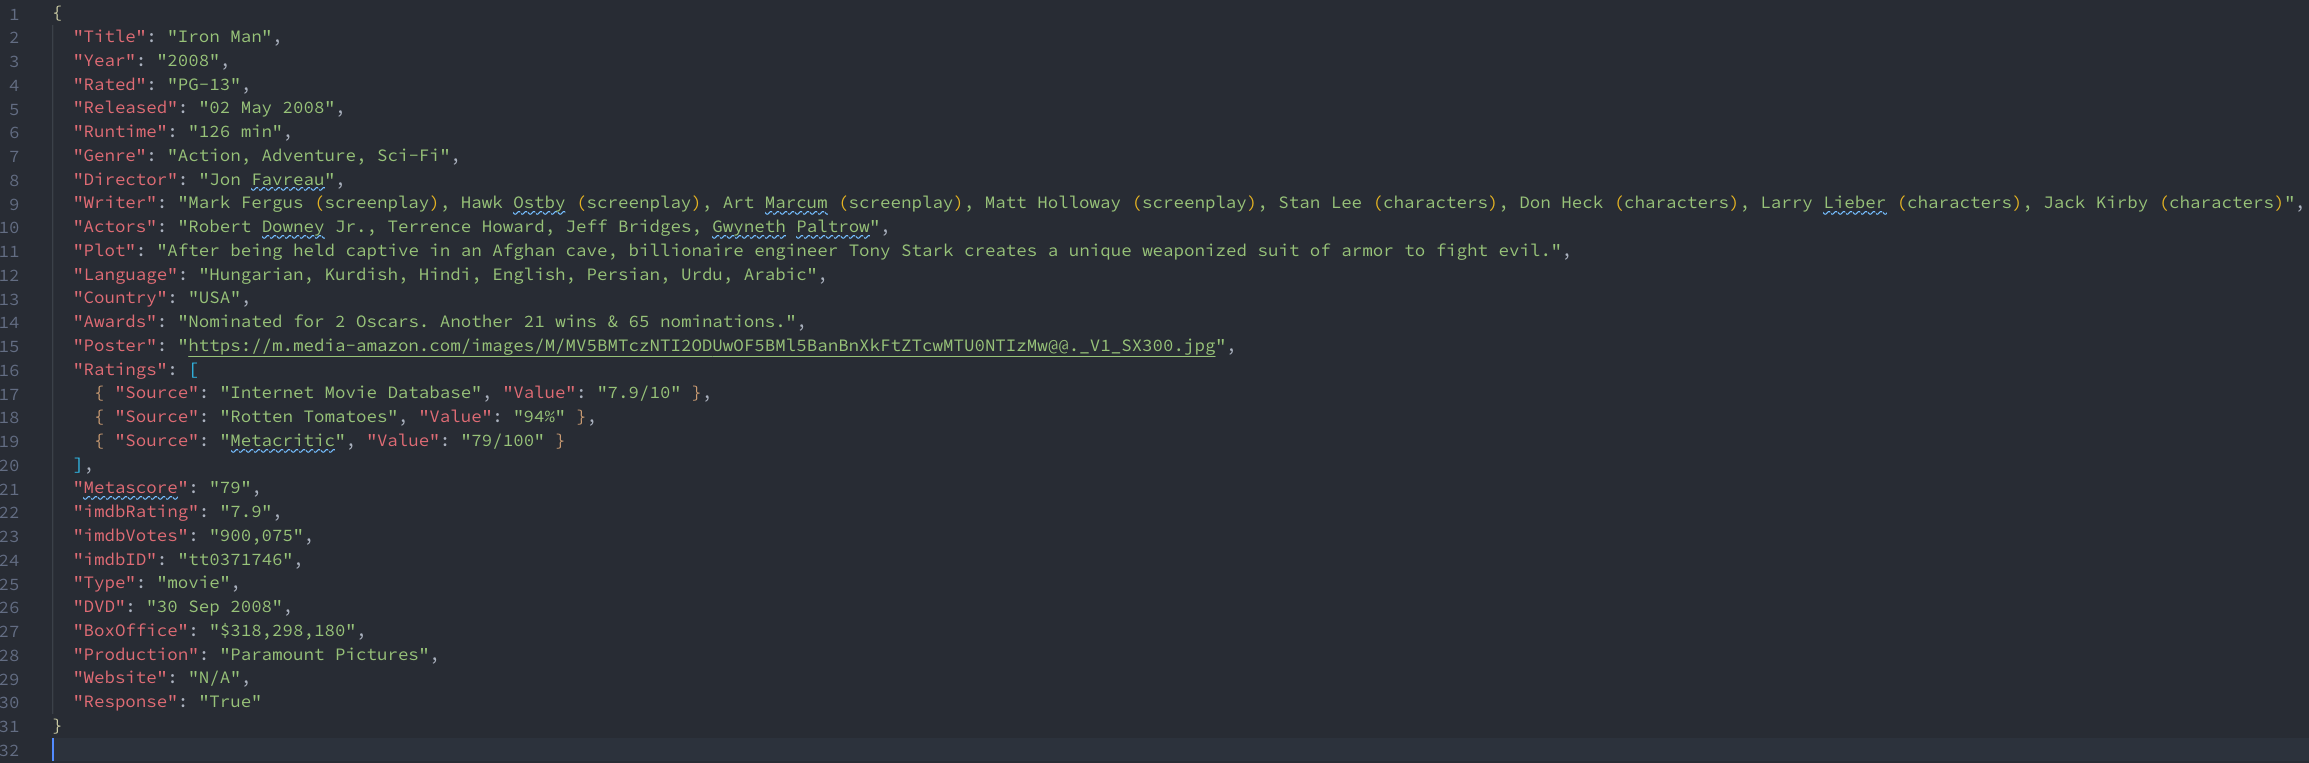
\includegraphics[width=100mm]{ironManJson.png}
                %     \caption{JSON returned for Iron Man}
                %     \label{fig:ironmanjson}
                % \end{figure}

        

                \begin{figure}[!htb]
                    \includegraphics[scale=0.25]{ironManObjects.png} 
                    \caption{Objects created by the importer for the movie Iron Man 2008}
                    \label{fig:ironManObjects}
                \end{figure}



                After each object has been created and stored, we can use the code in figure \ref{fig:CreatingExplanations} with a user id and the iron man movie id. This will give us the common objects between the user's profile and the movie. This is shown in figure \ref{fig:ironManObjectsCount}


                \begin{figure}[!htb]
                    \includegraphics[scale=0.25]{ironManObjectsCount.png} 
                    \caption{Common objects between the user with id 611 and the movie Iron Man (2008)}
                    \label{fig:ironManObjectsCount}
                \end{figure}


                After these have been created, each one gets turned into an explanation. The information is stored in a Python object along with a string that can be printed out to the screen and a score for that object related to its count. 

                The system then takes each one of these explanations and ranks them by score and uses the best in the debate. When the user begins the debate the movie is shown on the screen and we can see the explanation underneath. In figure \ref{fig:ironManSelection} we show the explanations that would be given if iron Man had won with its six explanations. The explanations are shown ordered by decreasing the score. 

                \begin{figure}[!htb]
                    \includegraphics[scale=0.4]{ironManSelection.png} 
                    \caption{The explanations produced by the system and shown with the movie Iron Man (2008)}
                    \label{fig:ironManSelection}
                \end{figure}

                We also had the ability to create explanations and score them with a random function. This produced the debate show in figure \ref{fig:ironManSelectionRandom}.

                \begin{figure}[!htb]
                    \includegraphics[scale=0.4]{ironManSelectionRandom.png} 
                    \caption{The randomly scored explanations shown with the movie Iron Man (2008)}
                    \label{fig:ironManSelectionRandom}
                \end{figure}

            
            \subsection{Critique}
                The focus of this system was to get it working so that a user could participate in the debate. In some of the rounds, we do not show the title or the poster of the movie. This can lead to some confusion as we have to refer to the movies from the selection box. A better way to do  this would be to place a button near each movie that would let you remove that one. The scoring of the explanations can sometimes lead to items that are not the best explanations being used. A better algorithm could have been created to calculate the usefulness of an explanation.


